\chapter{Referencial Teórico}
\label{chapter:Referencial_Teorico}

Neste capítulo, serão abordados os tópicos teóricos associados às redes sociais, aos grafos e à reutilização de software. Esses tópicos conferiram o embasamento teórico para realização deste trabalho.

\section{Redes Sociais}

Quando se pensa em rede, surge a ideia de um conjunto de nós interligados entre si, como uma teia que ocupa um determinado espaço em um ambiente. Os nós ou pontos estão ligados em pares e podem representar várias situações em áreas de interesse em comum \cite{Newman:2010}.

Para Sodré \cite{Sodre:2002}, rede é onde as conexões e as interseções tomam o lugar do que seria antes apenas linearidade. Essas conexões e interações ocorrem pelo contato direto, face a face, e pelo contato indireto, utilizando-se um veículo mediador, como o telefone.

As pessoas estão inseridas na sociedade por meio das relações que desenvolvem durante toda sua vida, primeiro no âmbito familiar, em seguida na escola, na comunidade em que vivem e no trabalho; enfim, as relações que as pessoas desenvolvem e mantêm fortalecem a esfera social. A própria natureza humana nos liga a outras pessoas, estruturando a sociedade em rede \cite{Tomae:Alcara:Chiara:2005}.

Os tipos de relações também podem ser de movimentação entre lugares, como migração, mobilidade física ou social; de conexão física, como uma estrada, um rio ou uma ponte que conecta dois lugares; de relações de autoridade, ou de relação biológica, como descendência, por exemplo \cite{Wasserman:1994}.

Com base em seu dinamismo, as redes, dentro do ambiente organizacional, funcionam como espaços para o compartilhamento de informação e conhecimento. Espaços que podem ser tanto presenciais quanto virtuais, em que pessoas com os mesmos objetivos trocam experiências, criando bases e gerando informações relevantes para o setor em que atuam \cite{Tomae:Alcara:Chiara:2005}.

\begin{quote}
	``[...] na era da informação – na qual vivemos – as
	funções e processos sociais organizam-se cada vez
	mais em torno de redes. Quer se trate das grandes
	empresas, do mercado financeiro, dos meios de
	comunicação ou das novas ONGs globais,
	constatamos que a organização em rede tornou-se
	um fenômeno social importante e uma fonte crítica
	de poder.'' \cite{Capra:2002}
\end{quote}

O contexto em que estamos inseridos desencadeia uma série de mudanças na rotina dos indivíduos, e uma delas evidencia as redes como ponto de convergência da informação e do conhecimento \cite{Tomae:Alcara:Chiara:2005}.

O conhecimento que a rede possui repercute sobre o meio que esta se encontra, pois Wellman \cite{Wellman:1996} verifica, na rede, sua identidade singular em determinada situação, isto é, a representação e a interpretação das relações em rede estão fortemente ligadas à realidade que a cerca; a rede é influenciada pelo seu contexto e esse por ela. Portanto, para \cite{Marteleto:2001}, os efeitos das redes podem ser percebidos fora de seu espaço, nas interações com o estado, na sociedade ou em outras instituições representativas.

A interação constante ocasiona mudanças estruturais e, em relação às interações em que a troca é a informação, a mudança estrutural que pode ser percebida é a do conhecimento. Quanto mais informação troca-se com o ambiente, com os atores da rede, maior será a bagagem de conhecimento, e maior será o estoque de informação, e é nesse conjunto de significados que se inserem as redes sociais \cite{Tomae:Alcara:Chiara:2005}.

Milgram, em sua tese \cite{Milgram:1967}, defende que qualquer pessoa está distante de qualquer outra pessoa do mundo, a no máximo seis graus de separação. Essa tese ficou conhecida como ``mundo pequeno'' e ``teoria dos seis degraus''. Sua pesquisa demonstra que a rede social constitui importante recurso profissional e pessoal. Estar em contato com pessoas que conheçam uma pessoa-alvo, em razão de um interesse específico, já é um passo além para a conquista de um objetivo.

\section{Teoria dos Grafos}

A análise de redes sociais tem como fundamento a teoria dos grafos. A seguir serão apresentados os principais conceitos sobre grafos.

\subsection{História}

O primeiro livro sobre a teoria dos grafos foi publicado por König (1936). Isso levou ao desenvolvimento de uma forte escola de teóricos em grafos na Hungria que incluíram P. Erdős e T. Gallai. Também na década de trinta, H. Whitney publicou uma série de artigos influentes \cite{Bondy:2007}.

De acordo com Ore \cite{Ore:1963}, Leonhard Euler\footnote{Grande matemático e físico suíço, 1707-1783, fez importantes descobertas em campos variados como Cálculo e Grafos.} teria sido um dos matemáticos mais importantes quando se refere a teoria dos grafos. Contam que o povo da cidade de Königsberg \footnote{Atualmente Caliningrado.}, localizado na Prússia e cortada pelo Rio Pregel, com sete pontes ligando duas ilhas e as margens opostas do rio, como pode ser visto na Figura \ref{Konigsberg}, propôs, ao então famoso matemático Leonard Euler, o seguinte problema:

	``Será possível fazer um passeio pela cidade, começando e
	terminando no mesmo lugar, cruzando cada ponte exatamente uma vez?''\cite{Ore:1963}

\begin{figure}[!h]
	\centering
	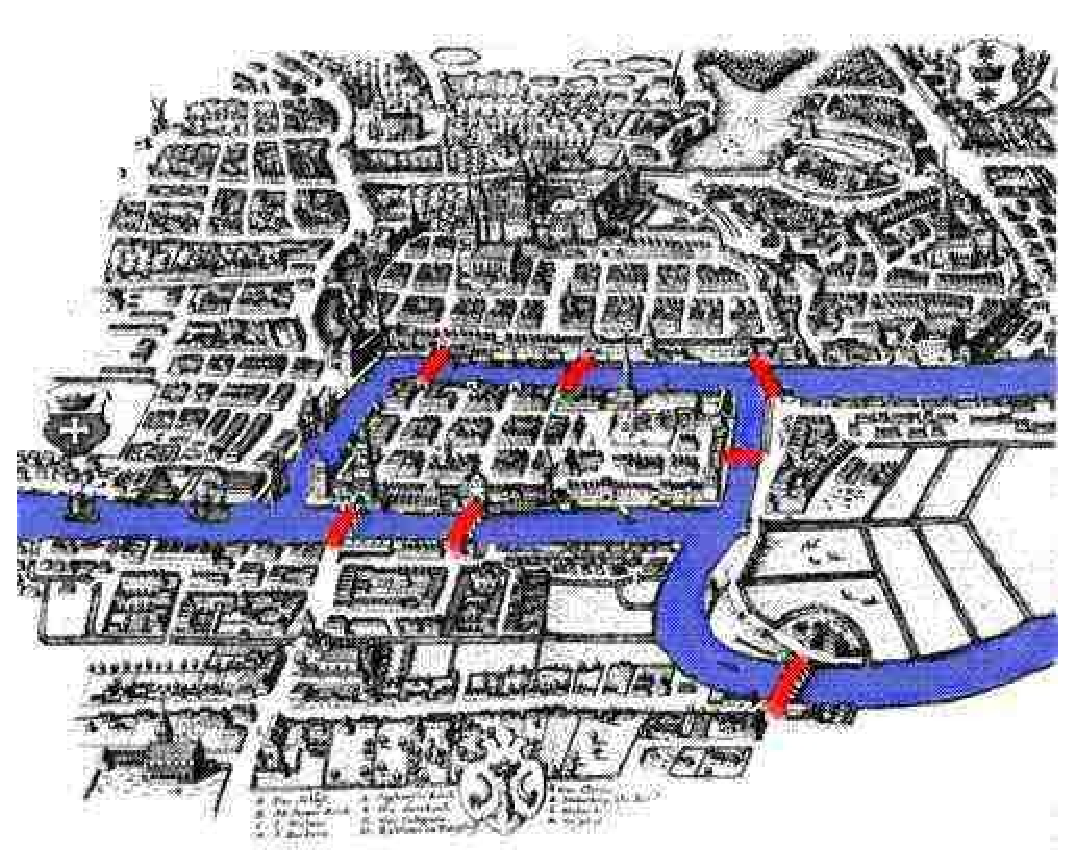
\includegraphics[scale=0.35]{figuras/referencial_teorico/Konigsberg.eps}
	\caption[Pontes de Königsberg]{Pontes de Königsberg\footnotemark}
	\label{Konigsberg}
\end{figure}
\footnotetext{\url{http://www.mat.uc.pt/~alma/escolas/pontes/}}

Não se tem conhecimento sobre o Euler ter resolvido esse problema usando a representação de grafos estudada hoje. A modelagem do problema por grafo passa por uma representação, na qual cada porção de terra  é representada por um ponto e as pontes estariam representadas por linhas \cite{Ore:1963}, conforme apresentado na Figura \ref{sete_pontes}.

\begin{figure}[!h]
	\centering
	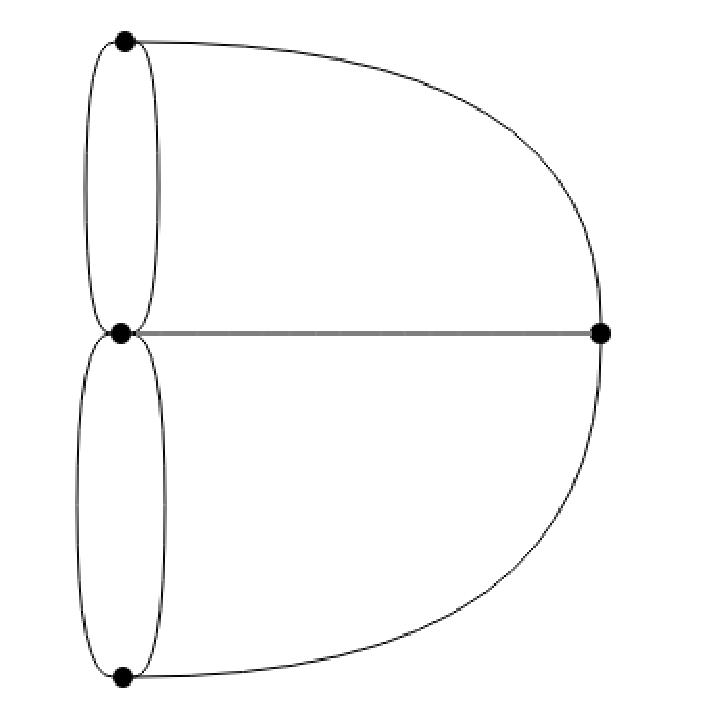
\includegraphics[scale=0.25]{figuras/referencial_teorico/sete_pontes.eps}
	\caption[Problema das sete pontes]{Problema das sete pontes \cite{Ore:1963}}
	\label{sete_pontes}
\end{figure}

Analisando, então, este problema, Euler resolveu a questão provando que uma caminhada assim é possível se, e somente se, o grafo for conectado e todos os seus vértices tiverem grau par, termos estes que serão tratados mais à frente \cite{Malta:2008}.

Assim, Euler mostrou que, uma vez que o grafo de Königsberg tem vértices de grau ímpar, a resposta ao problema era que tal caminhada era impossível. Desde então, todo grafo conexo, cujos vértices possuem grau par, é chamado de grafo euleriano, e um caminho fechado em um grafo que passe por cada aresta deste exatamente uma vez, é chamado de circuito (ou ciclo) euleriano \cite{Malta:2008}.

\subsection{Definições}

\textbf{Definição}: Um grafo é um par \textit{G} = (\textit{V}, \textit{E}) de conjuntos de tal modo que \textit{E}$\subseteq$[\textit{V}]$^2$. Assim, os elementos de \textit{E} são subconjuntos de pares ordenados de elementos de \textit{V}. Os elementos de \textit{V} são os vértices (ou nós ou pontos) do grafo \textit{G}, os elementos de \textit{E} são arestas (ou linhas) \cite{Diestel:1997}.

Grafos são assim chamados porque eles podem ser representados graficamente, e é esta representação gráfica que possibilita entender muitas de suas propriedades. Cada vértice é indicado por um ponto, e cada aresta por uma linha que une os pontos que representam as suas extremidades \cite{Bondy:2007}. Um exemplo pode ser observado na Figura \ref{exemplo_grafo}.

\begin{figure}[!h]
	\centering
	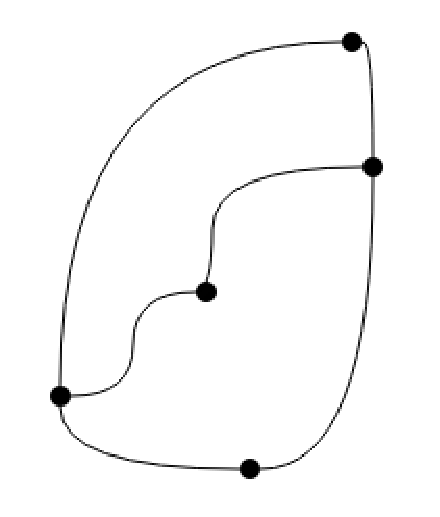
\includegraphics[scale=0.3]{figuras/referencial_teorico/exemplo_grafo.eps}
	\caption[Exemplo de grafo]{Exemplo de grafo \cite{Bondy:2007}}
	\label{exemplo_grafo}
\end{figure}

A maioria das definições e dos conceitos na teoria dos grafos são sugeridos por esta representação gráfica. As extremidades de uma aresta são referidas como sendo incidentes com a aresta, e vice-versa. Dois vértices que são incidentes com uma aresta em comum são chamados de adjacentes, e dois vértices adjacentes distintos são chamados de vizinhos \cite{Costa:2011}.

\subsection{Representação de Grafos}

Embora desenhos são um meio conveniente de especificação de grafos, eles claramente não são adequados para armazenar grafos em computadores, ou para a aplicação de métodos matemáticos para estudar suas propriedades. Para estes fins, são consideradas duas matrizes associadas com um grafo; uma matriz de incidência e uma matriz de adjacência \cite{Bondy:2007}.

Seja \textit{G} um grafo, com conjunto de vértices \textit{V} e conjunto de arestas \textit{E}. A matriz de incidência de \textit{G} é a matriz $M_G:= (m_{ve})$, com dimensões \textit{n$\times$m}, onde $m_{ve}$ é o número de vezes que o vértice \textit{v} e a aresta \textit{e} estão conectados \cite{Bondy:2007}.

A matriz de adjacência de \textit{G} é a matriz $A_G := (a_{uv})$, com dimensões \textit{n$\times$n}, em que $a_{uv}$ é o número de arestas que unem os vértices \textit{u} e \textit{v}. É possível verificar que a quantidade de memória necessária para essa representação é $\Theta(|\textit{V}|^2)$ \cite{Bondy:2007}. A Figura \ref{matriz} ilustra um grafo \textit{G} representado na matriz de incidência \textit{M} e na matriz de adjacência \textit{A}.

\begin{figure}[!h]
	\centering
	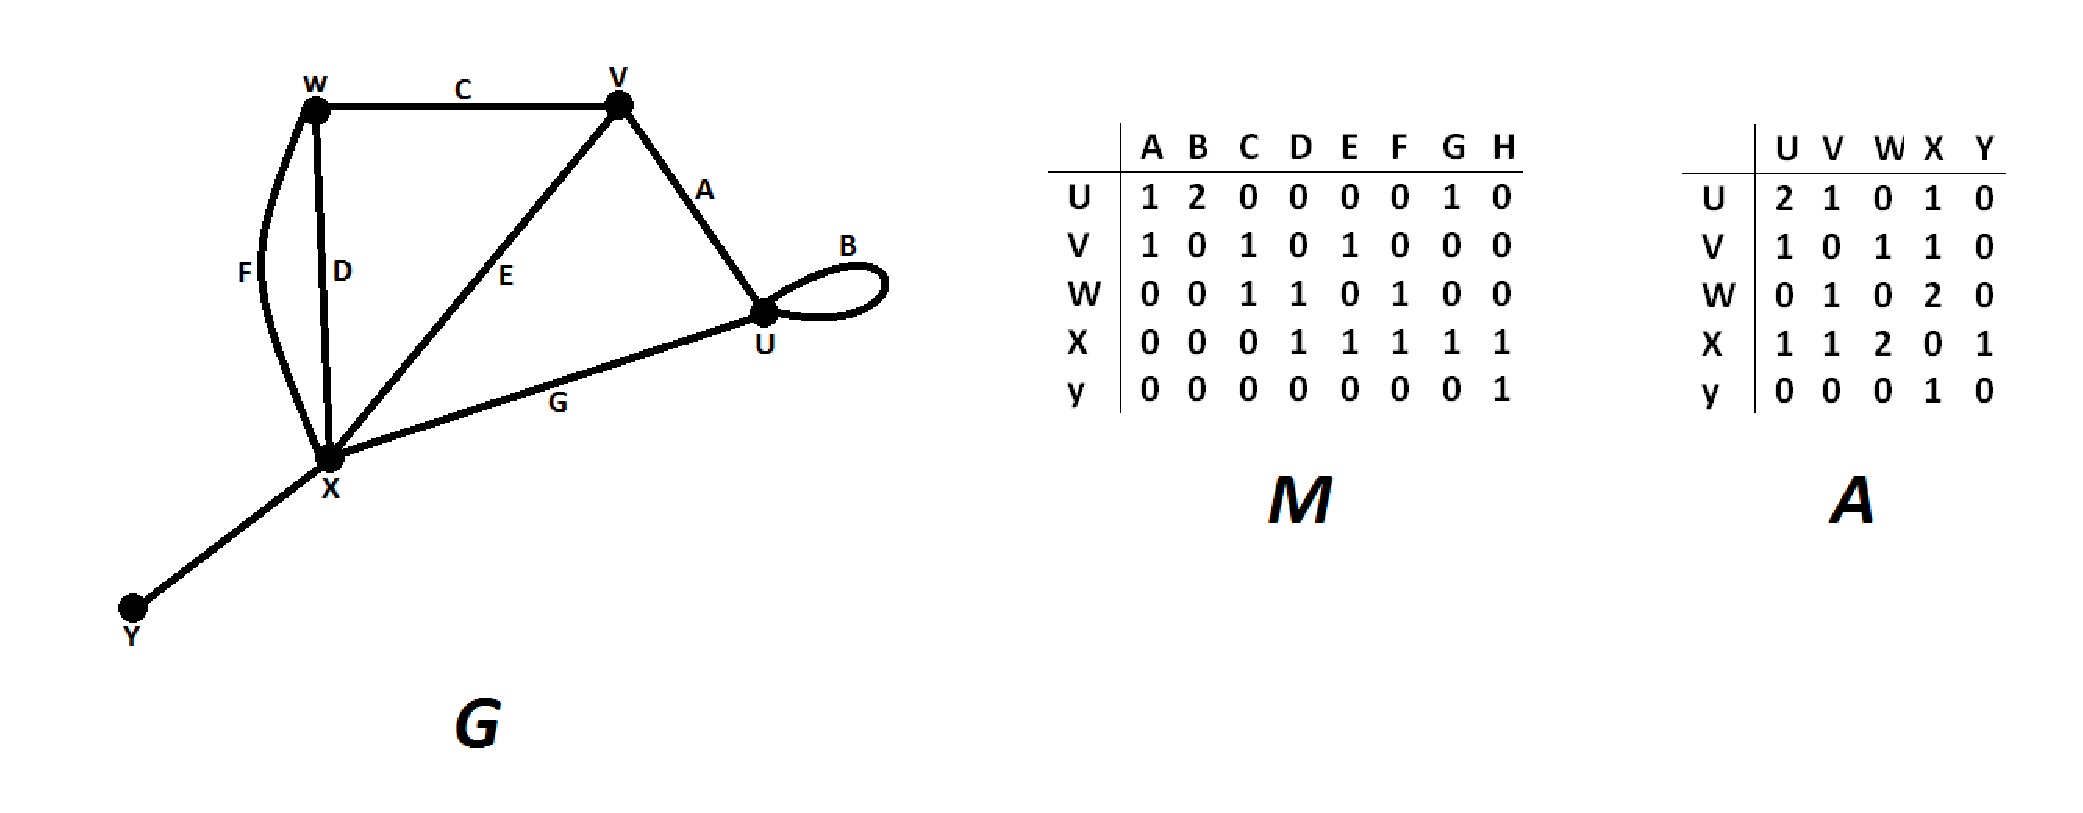
\includegraphics[scale=0.45]{figuras/referencial_teorico/matriz.eps}
	\caption[Representação em matriz]{Representação em matriz \cite{Bondy:2007}}
	\label{matriz}
\end{figure}

Como a maioria dos grafos possui um número bem maior de arestas do que os vértices, a matriz de adjacência de um grafo geralmente é menor do que a sua matriz de incidência e, assim, necessita de menos espaço de armazenamento. Ao lidar com grafos, é possível utilizar uma representação otimizada. Para cada vértice \textit{v}, os vizinhos de \textit{v} são armazenados em uma lista. A lista (\textit{N}(\textit{v}): \textit{v $\in$ V}) é chamada de lista de adjacência do grafo, onde \textit{N}(\textit{v}) representa os vizinhos do vértice \textit{v}. Um exemplo pode ser observado na Figura \ref{lista_adjacencia}. A quantidade de memória necessária para uma lista de adjacências é $\Theta(|\textit{V}| + |\textit{E}|)$. Grafos são, normalmente, armazenados em computadores como listas de adjacência. Entretanto, em casos em que o grafo possua muitos vértices e poucas arestas, a representação em matriz de incidência é eficiente. O mesmo acontece para a representação em matriz de de adjacência, quando o grafo possui poucos vértices e muitas arestas \cite{Costa:2011}.

\begin{figure}[!h]
	\centering
	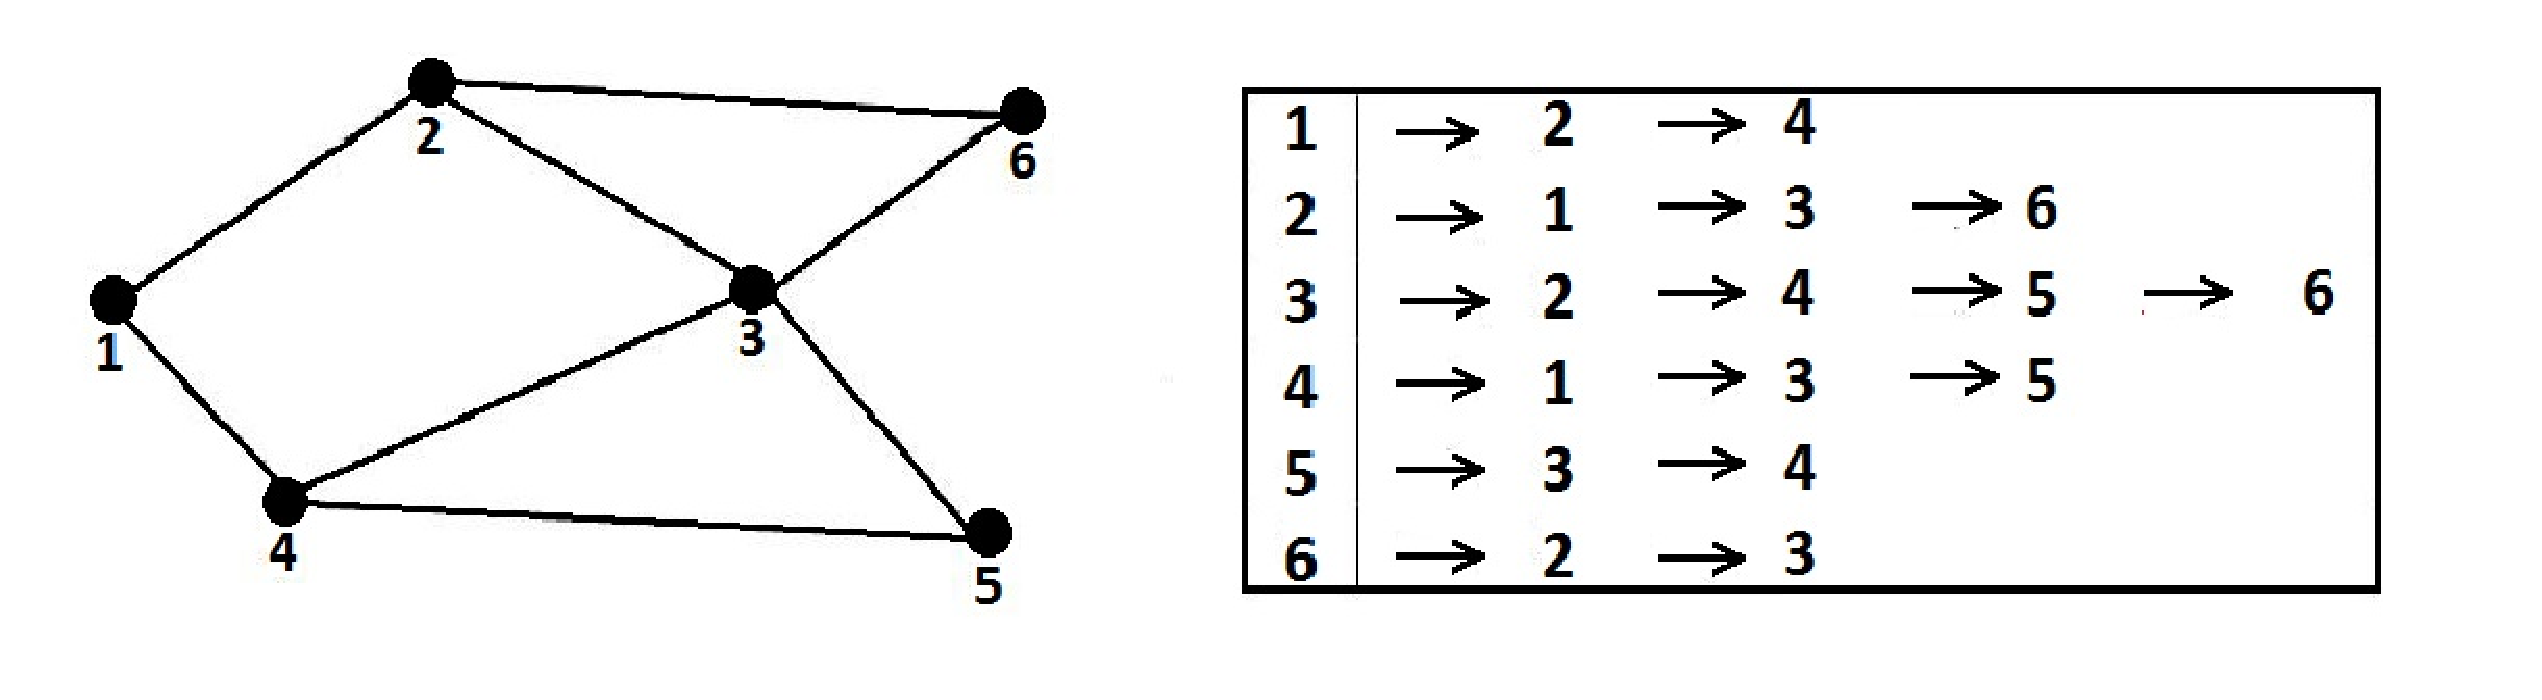
\includegraphics[scale=0.3]{figuras/referencial_teorico/lista_adjacencia.eps}
	\caption[Representação em lista de adjacência]{Representação em lista de adjacência \cite{Costa:2011}}
	\label{lista_adjacencia}
\end{figure}

Um conceito que torna-se muito importante ao se trabalhar com algoritmos complexos é a complexidades desses algoritmos, e como estes irão se comportar em uma aplicação. Certas complexidades podem tornar um algoritmo impraticável, a depender do caso. A seguir é apresentado um pouco mais sobre aspectos de complexidade de algoritmos.

\section{Complexidade de algoritmos}
\label{sec:complexidade_algoritmos}

Quando existem vários algoritmos que podem solucionar um problema, qual se deve escolher? Uma opção pode ser os algoritmos que possuem um fácil entendimento e depuração, porém dependendo do tipo de aplicação em que o algoritmo irá rodar, utilizar algoritmos que fazem um uso eficiente dos recursos do computador é essencial.

Para determinar qual algoritmo é mais eficiente que outro em determinado quesito, deve-se utilizar o cálculo de suas complexidades (custo). Este custo pode ser referente ao tempo de sua execução ou ao seu consumo de memória \cite{Albuquerque:2004}.

Para o cálculo de complexidade, pode-se medir o número de passos de execução em um modelo matemático denominado maquina de Turing, ou medir o número de segundos gastos em um computador específico. A medida de complexidade é o crescimento assintótico dessa contagem de operações \cite{Junior:2014}.

A objetivo de se fazer a análise de complexidade de um algoritmo é obter estimativas de tempos de execução do algoritmo \cite{Junior:2014}.

\subsection{Big O}

Uma das preocupações com a eficiência é com problemas que envolvem um grande número de elementos. Se existir uma tabela com apenas dez elementos, mesmo o algoritmo considerado menos eficiente resolvem o problema, no entanto, à medida que o número de elementos aumenta, o esforço necessário começa a fazer diferença de algoritmo para algoritmo. A notação \textit{Big O} faz uma estimativa de uma função de como o algoritmo se comporta com um número de elementos fixo ou tendendo ao infinito \cite{Junior:2014}. Pode-se observar na Figura \ref{grafico_complexidade} as principais funções que são utilizadas nesta notação.

Por exemplo, é mais importante saber que o número de operações executadas num algoritmo dobra se dobrarmos o valor de n, do que saber que para n igual a 100 são executadas 300 operações \cite{Junior:2014}.

\begin{figure}[!h]
	\centering
	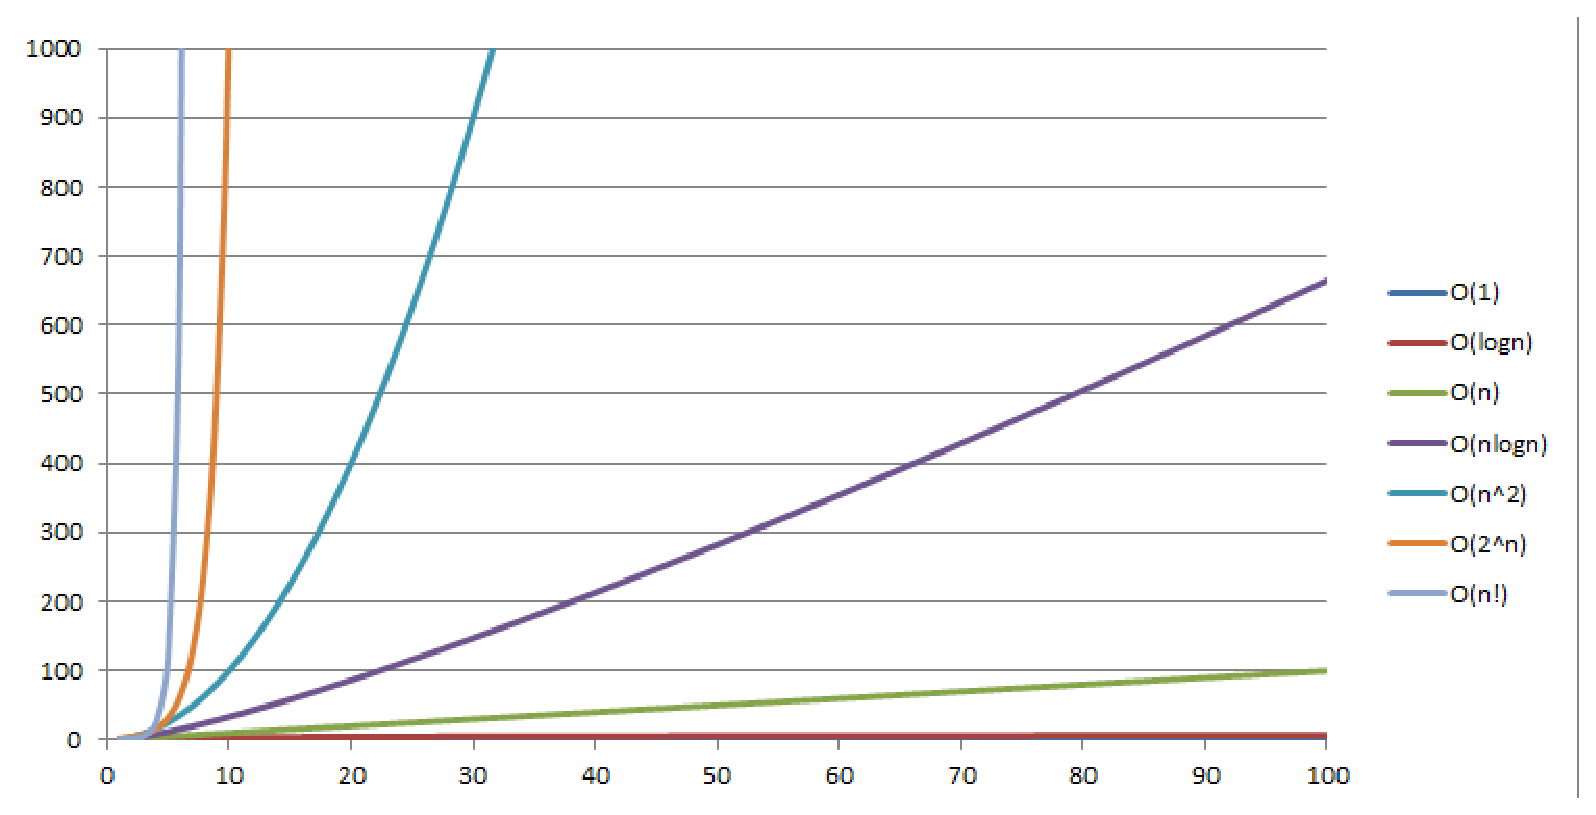
\includegraphics[scale=0.5]{figuras/apendices/grafico_complexidade.eps}
	\caption[Complexidade Big O]{Complexidade Big O}
	\label{grafico_complexidade}
\end{figure}

Os resultados expressos em notação \textit{Big O} devem ser interpretados com cuidado, pois indicam apenas que o tempo de execução do programa é proporcional a um determinado valor ou que nunca supera determinado valor. Na realidade o tempo de execução pode ser inferior ao valor indicado e pode ser que o pior caso nunca ocorra \cite{Junior:2014}.

Além dos conceitos de grafos e complexidade apresentados, este trabalho propõe-se também a trabalhar bastante com conceitos de \nameref{sec:reutilizacao_software}, a seguir serão apresentados alguns, dos principais contextos desse tema.

\section{Reutilização de Software}
\label{sec:reutilizacao_software}

A reutilização de software tem como objetivos aumentar a qualidade e a produtividade no desenvolvimento, pois busca evitar duplicidade de código e do esforço aplicado para desenvolver determinadas tarefas, reaproveitando o máximo possível experiências passadas \cite{Lucredio:2009}.

Todas as formas de reutilização de software usam algum tipo de abstração.  Essa é uma característica importante presente nas técnicas de reutilização, pois facilita aos desenvolvedores o uso de objetos reutilizáveis. Sem abstrações, os desenvolvedores deveriam analisar todos os artefatos reutilizáveis buscando entender como cada um funciona e como e quando devem ser utilizados \cite{Krueger:1992}.

Os próximos subtópicos irão apresentar temas deste trabalho que estão diretamente relacionados à reutilização de software.

\subsection{Frameworks}

\textit{Frameworks} compartilham técnicas de reutilização em geral e são considerados uma importante parte da cultura de desenvolvimento no mundo da orientação a objetos \cite{Johnson:1997}.

Fayad e Schimidt, em seu artigo \cite{Fayad:Schimidt:1997} sobre \textit{frameworks} de aplicações orientadas a objetos, mostram quais são os principais benefícios no uso de \textit{frameworks}, dentre eles: modularização, reutilização, extensibilidade e inversão de controle.

\begin{itemize}
	\item \textbf{modularização:} \textit{Frameworks} encapsulam e interfaceiam alguns detalhes de implementação. Isso reduz o esforço necessário para entender e manter partes do software existente, pois basta ao desenvolvedor usar o que lhe é oferecido sem necessariamente entender qual a implementação do \textit{framework};

	\item \textbf{reutilização:} As interfaces providas por \textit{frameworks} ajudam também na reutilização através da definição de componentes genéricos, que podem ser aplicados em outras aplicações. Assim sendo, soluções comuns para sistemas diferentes podem ser usadas da mesma forma sem a necessidade de recriação das mesmas. Entende-se então, que estas soluções são pensadas uma única vez, e ao estarem presentes em um \textit{framework}, basta que sejam usadas;

	\item \textbf{extensibilidade:} Este é um dos principais pontos positivos dos \textit{frameworks}, pois estes fornecem métodos e interfaces estáveis que outras aplicações irão utilizar. Recomenda-se que essas aplicações façam uso desses métodos, visando resolver problemas parecidos em diferentes contextos. Uma boa estrutura de extensibilidade é essencial para garantir a customização de novos serviços e funcionalidades das aplicações, e;

	\item \textbf{inversão de controle:} A inversão de controle ocorre devido a forma como serão processados e entendidos muitos dos eventos de uma aplicação, que ficam invisíveis ao desenvolvedor quando este usa um \textit{framework}, pois é o próprio \textit{framework} quem decide o conjunto de métodos que será invocado para realizar uma determinada tarefa da aplicação.
\end{itemize}

\subsubsection{Frameworks e Reutilização de Software}

A tecnologia de reutilização ideal provê componentes que podem facilmente ser conectados para criar um novo sistema. Não é necessário ao desenvolvedor - cliente do framework - ter conhecimento de como o componente é implementado, e geralmente é fácil para ele aprender como o utilizar. O resultado é que o sistema tende a ser eficiente, fácil de manter e confiável \cite{Johnson:1997}.

\textit{Frameworks} são aplicações especializadas em prover classes e componentes abstratos que podem ser usados por outros sistemas. Estes proveem técnicas de reutilização robustas e de maior granularidade. Sendo aplicações independentes, é mais fácil usá-los em um maior número de sistemas \cite{Johnson:Foote:1988}.

Para se alcançar a aplicação efetiva de um dado \textit{framework}, é necessário ao desenvolvedor conhecer as interfaces que o \textit{framework} proporciona antes de poder usá-las. Como podem existir diversas interfaces complexas, aprender a usar um novo \textit{framework} pode ser difícil. Porém, os \textit{frameworks} são poderosos e o tempo gasto em sua aprendizagem tende a ser recompensado, pois podem reduzir a quantidade de esforço aplicado para se desenvolver uma nova aplicação que os use \cite{Johnson:1997}.

Ao longo do tempo, tornou-se muito caro desenvolver aplicações complexas a partir do zero. Isso ocorre, pois os componentes que são desenvolvidos devem passar por um criterioso processo de validação e manutenção, e isso procede sempre que um novo sistema é desenvolvido. Ao se usar \textit{frameworks}, pode-se desenvolver componentes comuns e os processos citados são feitos em um único local \cite{Fayad:Schimidt:1997}.

As técnicas de reutilização são diferentes de acordo como o tipo do \textit{framework} utilizados. Esses tipos podem ser ``\textit{white box}'' ou ``\textit{black box}''. O primeiro diz respeito a quando o código do \textit{framework} é aberto e visível ao desenvolvedor, dessa forma, este pode estudar a implementação do \textit{framework} e modificar o código de determinadas partes de acordo com suas necessidades. Os \textit{frameworks} do tipo ``\textit{black box}'' disponibilizam apenas interfaces ao desenvolvedor para que este possa usá-las. A forma como tudo é implementado e processado é desconhecida. No primeiro tipo, têm-se uma maior flexibilidade, porém, o uso é mais complexo ao desenvolvedor. No segundo, o uso é bem simples, porém, não existe flexibilidade para mudança da implementação \cite{Kroth:2000}.

Existe também uma metodologia no desenvolvimento de \textit{frameworks} que une as técnicas ``\textit{white box}'' e ``\textit{black box}'', assim, uma parte do \textit{framework} é fechada e o desenvolvedor não pode alterar o código, apenas usar as funções disponíveis; outra parte é aberta ao desenvolvedor para realizar alterações no código. Essa abordagem é conhecida como \textit{frameworks} do tipo ``\textit{gray box}'' ou ``caixa cinza'' \cite{Kristensen:2004}.

Além dos tipos de \textit{frameworks}, estes também podem ser divididos quanto a sua aplicabilidade. Podem ser desenvolvidos para serem aplicados em qualquer domínio, de forma genérica sem se preocupar com algo específico, \textit{frameworks horizontais}; ou podem ser desenvolvidos visando atender um tipo específico de domínio de problemas, \textit{frameworks verticais}. Essas características dependem das necessidades apresentadas ao se trabalhar com \textit{frameworks}, e isso impacta como será aplicada a reutilização \cite{Kroth:2000}.

Na engenharia de software, busca-se cada vez mais o aumento da produtividade e da qualidade dos sistemas desenvolvidos. A reutilização de software, ao contrário de todas as demais partes de um sistema, é um fator que pode acarretar o aumento desses fatores, considerando que, ao se utilizar componentes já desenvolvidos e depurados, pode-se reduzir o tempo de desenvolvimento, de testes e as chances de ocorrência de erros que poderiam advir se fosse necessária a criação destes novos artefatos \cite{Silva:2000}.

Na qualidade, a reutilização advinda dos \textit{frameworks} pode trazer ganhos de desempenho, confiabilidade e interoperabilidade de software \cite{Fayad:Schimidt:1997}.

\subsubsection{Frameworks e Padrões}

Padrões representam soluções recorrentes para problemas no desenvolvimento de software em um contexto específico. Tanto os padrões como os \textit{frameworks} são técnicas de reutilização. A grande diferença é que os \textit{frameworks} concentram-se na reutilização de estruturas, algoritmos e implementações em uma dada linguagem de programação. Já os padrões focam em apresentar desenhos abstratos de como resolver problemas; como microarquiteturas de software \cite{Fayad:Schimidt:1997}.

Um padrão descreve um problema a ser resolvido, apresenta uma solução e o contexto em que essa solução funciona, nomeia uma técnica, e descreve seus custos e benefícios \cite{Johnson:1997}.

Quando um \textit{framework} é implementado diversas vezes, este também pode ser considerado um padrão \cite{Johnson:1997}. O MVC (\textit{Model / View / Controller}) é um \textit{framework} conceitual de interface com usuário que é considerado um padrão arquitetural\cite{Almeida:2006}.

Segundo \cite{Fayad:Schimidt:1997}, quando usados em conjunto com padrões, os \textit{frameworks} podem aumentar significativamente a qualidade do software e reduzir o esforço de desenvolvimento.

\subsection{Padrões de Projeto}

Os padrões de Projeto são parte da vanguarda da tecnologia orientada a objetos, e este tema tem estado em constante crescimento no decorrer dos tempos\cite{Shalloway:Trott:2004}. A proposição por trás dos padrões é que a qualidade do software pode ser medida objetivamente. Tal fato considera que, ao se analisar, o \textit{design} de um padrão, este pode ser considerado bom ou ruim, e assim resultando em uma qualidade adequada ou inadequada\cite{Shalloway:Trott:2004}.

Alexander, em seu livro \cite{Alexander:1979} sobre padrões de construção, diz:

\begin{quote}
	``Cada padrão descreve um problema no nosso
ambiente e o cerne da sua solução, de tal forma que você possa usar essa solução mais
de um milhão de vezes, sem nunca fazê-lo da mesma maneira.''
\end{quote}

No livro de padrões de projeto \cite{Gamma:1995}, os autores concordam com as afirmações de Alexander. A diferença principal é que, no âmbito de software, os padrões são expressos em termos de objetos e interfaces ao invés de paredes e portas. Porém, ambos os tipos de padrões dizem respeito à solução para um problema em um contexto geral. Os autores consideram ainda que um padrão é dividido em quatro partes principais, que são:

\begin{itemize}
	\item \textbf{nome:} Usado para descrever um problema de projeto, suas soluções e consequências em uma ou duas palavras. Quando um padrão possui um nome fica mais fácil de definir um vocabulário comum para tratar deste com outras pessoas;
	\item \textbf{problema:} O problema está ligado diretamente à situação em que deve ser aplicado o padrão, ou seja, qual o contexto. Algumas vezes o problema pode conter uma lista de condições que devem ser satisfeitas para que se possa alcançar sentido na aplicação do padrão;
	\item \textbf{solução:} Esta descreve todos os elementos que compõem o padrão, seus relacionamentos, responsabilidades e colaborações. É fornecida uma descrição abstrata de um problema de projeto e o arranjo geral de classes e objetos que resolvam o padrão. Não há uma solução ou implementação concreta, pois padrões são desenhados para serem usados em diferentes situações, e;
	\item \textbf{consequências:} As consequências apresentam uma série de resultados concernentes da aplicação do padrão, normalmente apresentando vantagens e desvantagens. São elementos críticos que entram na decisão da aplicação ou não do padrão que está em questão.
\end{itemize}

\subsubsection{Por que usar Padrões de Projeto?}

Os três pontos que justificam de forma adequada o uso de padrões de projeto são brevemente descritos a seguir, de acordo com \cite{Shalloway:Trott:2004}:

\begin{itemize}
	\item \textbf{soluções reutilizáveis:} O tempo gasto para aprender a utilizar determinado padrão é compensado pela reutilização que é oferecida. Têm-se o benefício de aplicar o que foi aprendido para diversos projetos. Depois de ter o conhecimento fixado, não é necessário reinventar soluções para problemas recorrentes, basta reutilizar o que os padrões oferecem;
	\item \textbf{terminologia comum:} Quando se está em um grupo de trabalho, são necessários uma base de vocabulário e pontos de visão do problema comuns. Os padrões de projeto providenciam um ponto comum de referência durante as fases de análise e \textit{design} de um projeto, e;
	\item \textbf{perspectiva de alto nível do problema:} Os padrões dão aos desenvolvedores essa perspectiva, e ajudam na análise e entendimento dos problemas, facilitando a elaboração de uma solução mais adequada.
\end{itemize}

Os padrões ainda podem ajudar na refatoração de projetos. Uma das grandes dificuldades no desenvolvimento de software é que este tem de ser frequentemente reorganizado ou refatorado. Os padrões de projeto, ao oferecerem soluções comuns e já consolidadas, podem reduzir a quantidade de refatoração que deverá ser feita mais tarde \cite{Gamma:1995}.

\subsubsection{Classificação de Padrões de Projeto}

Em \cite{Gamma:1995}, foram definidos e classificados 23 padrões. Essa classificação está feita de acordo com dois critérios: \textbf{finalidade} e \textbf{escopo}. O primeiro critério diz respeito ao que o padrão faz. A finalidade pode ser de criação, estrutural ou comportamental. Os padrões com finalidade de criação se preocupam com o processo de criação de objetos. Os estruturais focam em composições de classes ou objetos. Os comportamentais caracterizam as maneiras que as classes ou objetos interagem e distribuem responsabilidades.

O segundo critério especifica se o padrão é de classe ou objeto. Os padrões de classe lidam com relacionamentos entre classes e suas subclasses, para isso são utilizados relacionamentos de herança. E os padrões de objetos são mais dinâmicos, pois lidam com relacionamentos entre objetos que podem ser mudados em tempo de execução.

Nos apêndices em \nameref{chapter:reutilizacao_software} são encontrados alguns outros aspectos de reutilização, como serviços e o detalhamento de três padrões de projeto que foram implementados no desenvolvimento deste trabalho.

\section{Resumo do Capítulo}
Este capítulo apresentou o levantamento bibliográfico dos temas relacionados ao desenvolvimento deste trabalho. A seguir são apresentados os temas descritos nesse capítulo.

\begin{itemize}
	\item Redes Sociais: este é o tema em que este trabalho é desenvolvido. Como o presente trabalho focou no desenvolvimento de um \textit{framework} para redes sociais, é essencial o conhecimento e o entendimento deste tema para a realização deste tema.
	\item Teoria dos Grafos: o desenvolvimento de redes sociais têm como base o uso de grafos e, sendo assim, este é também um tema de suma importância para este trabalho.
	\item Reutilização de Software: este tópico representa um importante objetivo investigado ao longo desse trabalho. A reutilização de software é apresentada no uso de \textit{frameworks}, padrões de projeto e serviços, todos estes utilizados na implementação do \textit{framework}.
\end{itemize}

Outros detalhes de alguns tópicos apresentados neste capítulo podem ser encontrados na parte de apêndices deste documento.

O próximo capítulo apresenta a metodologia usada no decorrer do desenvolvimento deste trabalho.
